\section{Objetivo}

  Tem como objetivo a identificação dos possíveis riscos envolvidos no projeto, tal como os planos para tratamento.

\section{Riscos}

  Todos os riscos já identificados e futuros riscos serão documentados e apresentados neste documento, contendo suas
  características e possíveis soluções.

\subsection{Processo de gerenciamento de riscos}

  Visa definir um processo para qual os membros da equipe de gerência devem seguir para controle dos riscos no projeto.

  \begin{table}[!htb]
    \centering
    \begin{tabular}{p{5cm}p{10cm}}
      \toprule
        \textbf{Processo} & \textbf{Descrição} \\
      \midrule
        Identificar riscos  & Visa identificar os riscos que podem atrapalhar o projeto                                         \\ \midrule
        Analisar riscos     & Visa planejar como os riscos que possam vir ocorrer serão controlados ou resolvidos.              \\ \midrule
        Controlar riscos    & Visa acompanhar os riscos durante o período do projeto, avaliando a forma de resolução dos mesmos
                              durante toda a vida útil do projeto.                                                              \\
      \bottomrule
    \end{tabular}
    \caption{Processo de gerenciamento de risco}
  \end{table}

\subsection{Tabela dos riscos encontrados}

  Todos os riscos encontrados que podem prejudicar de alguma forma o projeto.

  \begin{table}[!htb]
    \centering
    \begin{tabular}{p{5cm}p{5cm}p{5cm}}
      \toprule
        \textbf{Risco} & \textbf{Impacto} & \textbf{Principal causa} \\
      \midrule
        Greve da UnB                                                    & Cronograma do projeto afetado                                   & Professores ou alunos insatisfeitos                                                   \\ \midrule
        Desistência ou falta de comprometimento de membros do projeto   & Atividades precisarão ser realocadas entre os membros restantes & Desmotivação dos alunos com a disciplina                                              \\ \midrule
        Falha no planejamento do projeto                                & Projeto entregue incompleto no ponto de controle seguinte       & Inexperiência da equipe de gerência                                                   \\ \midrule
        Mudanças no escopo                                              & Ajustes em toda a documentação do projeto                       & Falha de planejamento por partes dos alunos ou solicitação por parte dos professores  \\ \midrule
        Não cumprimento do escopo estabelecido                          & Projeto final faltando informações                              & Falta de maturidade da equipe do projeto                                              \\ \midrule
        Atraso na entrega dos documentos para a elaboração do relatório & Diminuição da nota do projeto                                   & Falta de comprometimento por parte dos membros                                        \\ \midrule
        Plágio nos relatórios                                           & Diminuição da credibilidade do relatório                        & Falta de comprometimento por parte dos membros                                        \\ \midrule
        Legislação não permitir realizar certas tarefas                 & Terá que fazer mudanças no escopo do projeto                    & Restrições estabelecidas pelas leis                                                   \\
      \bottomrule
    \end{tabular}
    \caption{Tabela de riscos do projeto}
  \end{table}

\newpage

\section{Qualificação dos riscos}

\subsection{Probabilidade de impacto dos riscos}

  A seguir está a probabilidade de impacto dos riscos

  \begin{table}[!htb]
    \centering
    \begin{tabular}{p{5cm}p{3cm}p{3cm}}
      \toprule
        \textbf{Probabilidade} & \textbf{Intervalo} & \textbf{Peso} \\
      \midrule
        Muito baixo & 0 $-$ 20\%    & 1 \\ \midrule
        Baixo       & 21 $-$ 40\%   & 2 \\ \midrule
        Moderado    & 41 $-$ 60\%   & 3 \\ \midrule
        Alta        & 61 $-$ 80\%   & 4 \\ \midrule
        Muito alta  & 81 $-$ 100\%  & 5 \\
      \bottomrule
    \end{tabular}
    \caption{Probabilidade de impacto dos riscos}
  \end{table}

  O impacto mede o quão prejudicial um risco é ao projeto como um todo, a seguir, está demonstrado como o impacto será representado.

  \begin{table}[!htb]
    \centering
    \begin{tabular}{p{3cm}p{5cm}p{2cm}}
      \toprule
        \textbf{Impacto} & \textbf{Descrição} & \textbf{Peso} \\
      \midrule
        Muito baixo & Impacto no projeto não é expressivo           & 1 \\ \midrule
        Baixo       & Impacto pouco expressivo                      & 2 \\ \midrule
        Moderado    & Pode prejudicar o projeto de maneira moderada & 3 \\ \midrule
        Alta        & Prejudica o andamento do projeto              & 4 \\ \midrule
        Muito alta  & Prejudica gravemente o andamento do projeto   & 5 \\
      \bottomrule
    \end{tabular}
    \caption{Qual prejudicial é o nível do impacto}
  \end{table}

\section{Matriz de probabilidade de impacto}

  É utilizada para mapear os riscos de acordo com sua probabilidade de ocorrer e impacto no projeto, dando maior visão do que deve ser
  priorizado pela equipe.

  \begin{table}[!htb]
    \centering
    \begin{tabular}{cp{2cm}p{2cm}p{2cm}p{2cm}p{2cm}}
      \toprule
        \textbf{Probabilidade/Impacto} & \textbf{1} & \textbf{2} & \textbf{3} & \textbf{4} & \textbf{5} \\
      \midrule
        \textbf{1} & 1 & 2  & 3  & 4  & 5  \\ \midrule
        \textbf{2} & 2 & 4  & 6  & 8  & 10 \\ \midrule
        \textbf{3} & 3 & 6  & 9  & 12 & 15 \\ \midrule
        \textbf{4} & 4 & 8  & 12 & 16 & 20 \\ \midrule
        \textbf{5} & 5 & 10 & 15 & 20 & 25 \\
      \bottomrule
    \end{tabular}
    \caption{Matriz de probabilidade de impacto}
  \end{table}

  Com o resultado da matriz de probabilidade, temos a seguinte estratégia de gerenciamento de riscos.

  \begin{itemize}
    \item \textbf{Aceitação do risco}: Não fazer nada a respeito do risco, porém tentar resolver o problema que será gerado no projeto,
      isso significa que se o problema realmente acontecer, você vai lidar com ele, em vez de antecipar  qualquer esforço para impedir
      que ocorra.
    \item \textbf{Mitigação do risco}: Limitar o impacto de um risco agindo antes dele acontecer.
    \item \textbf{Prevenção do risco}: Evitar completamente o risco, trata-se de fazer mudanças (às vezes drásticas) em seu plano do
      projeto e cronograma, para evitar o problema em potencial.
  \end{itemize}

  \begin{table}[!htb]
    \centering
    \begin{tabular}{p{5cm}p{5cm}p{5cm}}
      \toprule
        \textbf{Nível de prioridade} & \textbf{Intervalo da matriz} & \textbf{Ação a ser tomada} \\
      \midrule
      Baixo & 1 $-$ 5   & Aceitação do risco \\ \midrule
      Médio & 6 $-$ 14  & Mitigação do risco \\ \midrule
      Alto  & 15 $-$ 25 & Prevenção do risco \\
      \bottomrule
    \end{tabular}
    \caption{Ação a ser tomada no risco}
  \end{table}

\section{Controle de riscos}

  \begin{figure}[!htb]
    \centering
    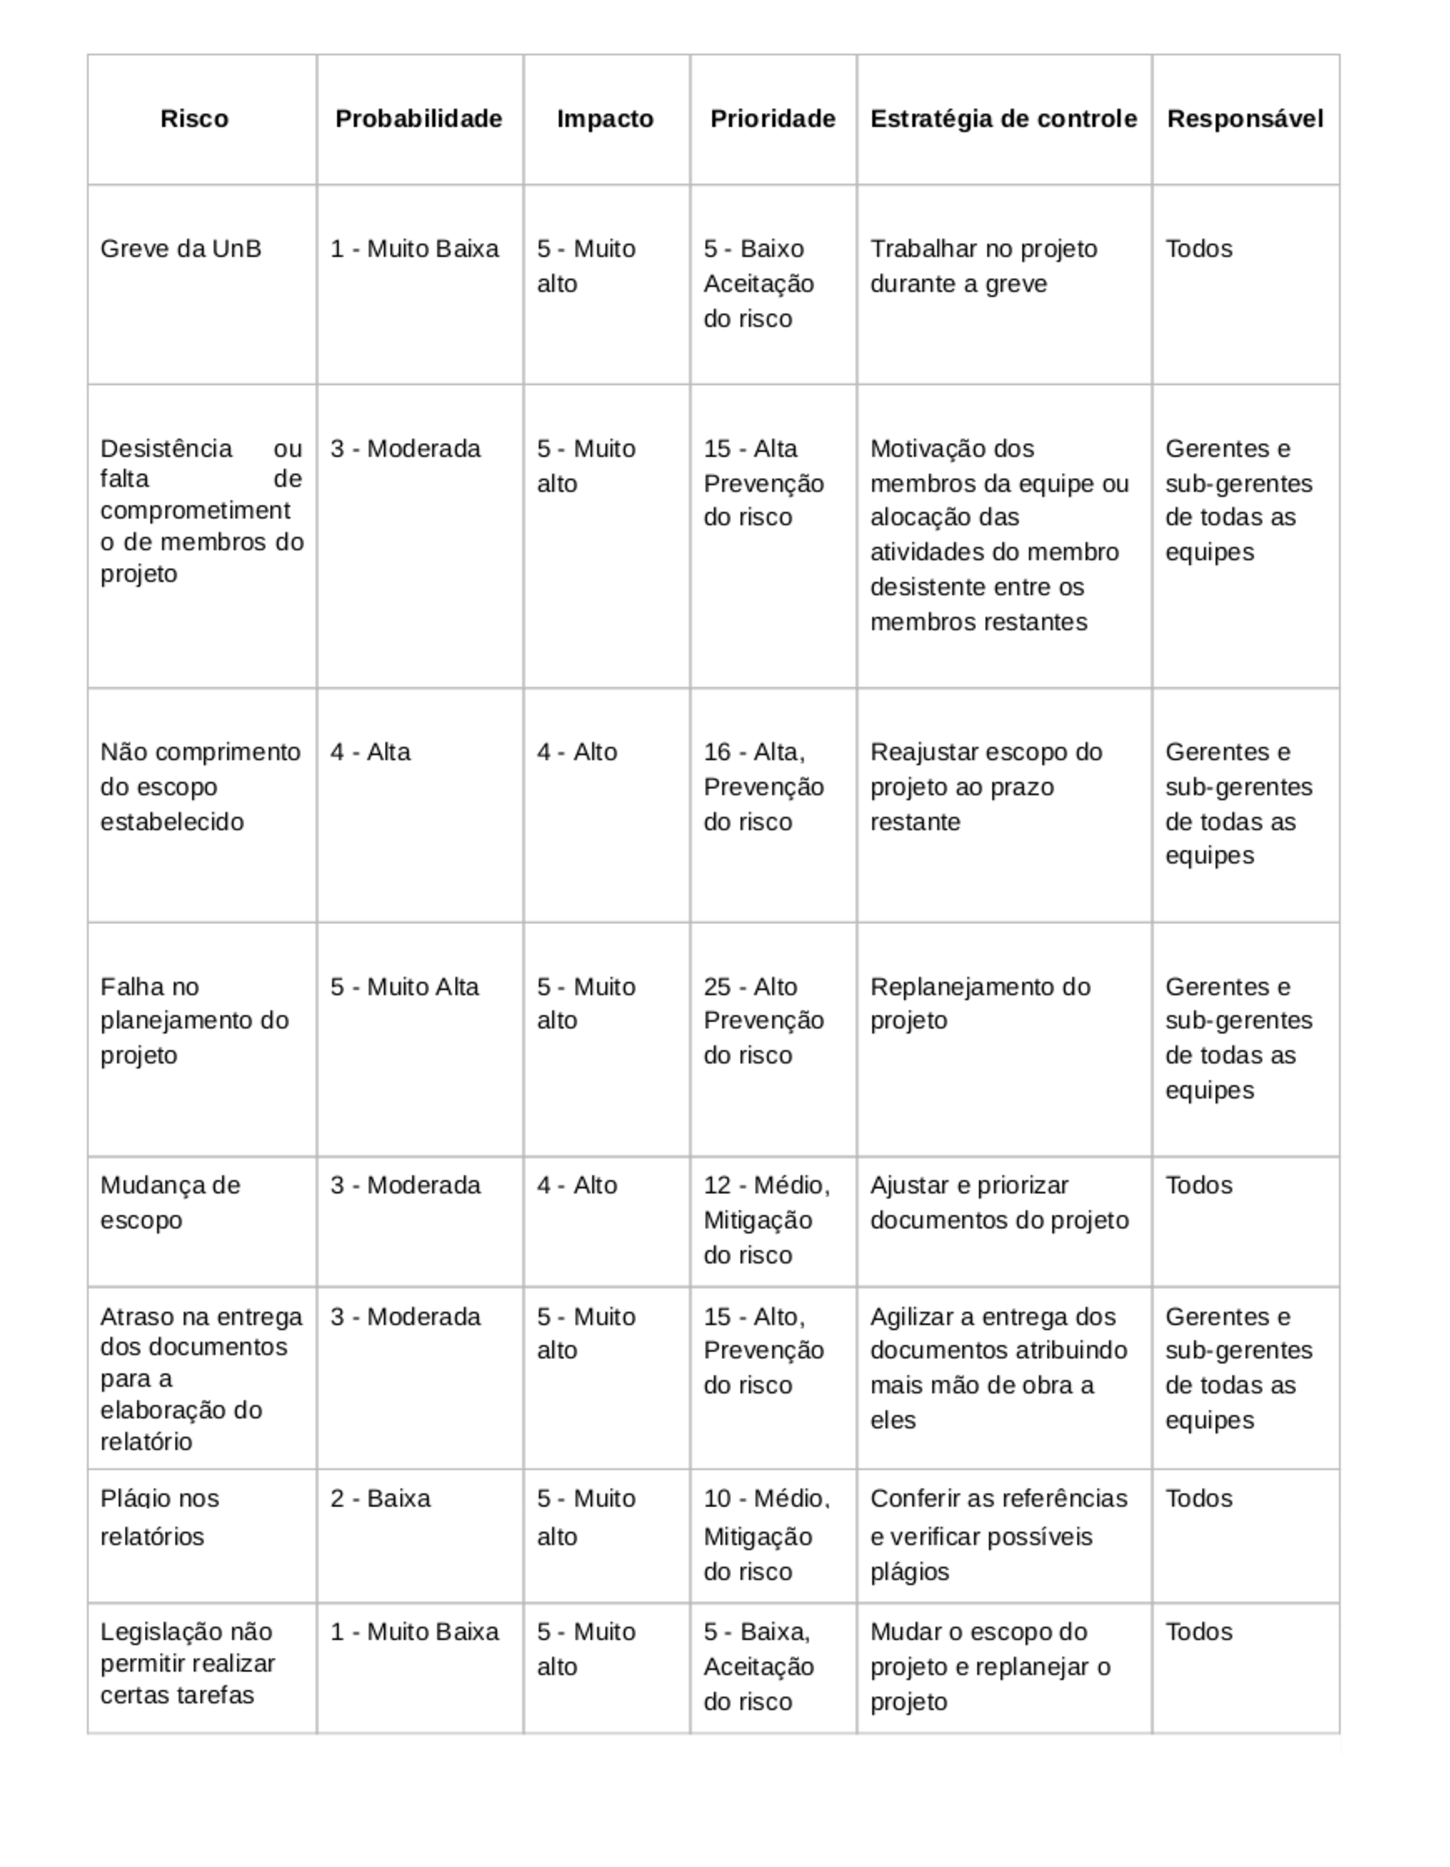
\includegraphics[width=15cm, keepaspectratio=true]{figuras/risco/risco.eps}
    \caption{Controle de riscos}
  \end{figure}

